\documentclass[conference]{IEEEtran}
\IEEEoverridecommandlockouts
\usepackage{cite}
\usepackage{amsmath,amssymb}
\usepackage{booktabs}
\usepackage{graphicx}
\usepackage{array}
\usepackage{url}
\usepackage{microtype}
\usepackage{tikz}
\usetikzlibrary{arrows.meta,positioning,shapes.geometric,fit,calc}
\usepackage{pgfplots}
\pgfplotsset{compat=1.18}

\title{AegisCloud: An Evidence-Guided Cloud Threat Detection and Risk-Triage Platform}

\author{\IEEEauthorblockN{Premanand Ghadekar, Tanmay Kumbhare, Hemantkumar~S.~Lakhane, Dhanashri Khode, Khushi Ghumre}
\IEEEauthorblockA{Department of Computer Science and Engineering (Artificial Intelligence and Machine Learning)\\
Vishwakarma Institute of Technology, Pune, India\\
\{premanand.ghadekar, tanmay.kumbhare24, hemantkumar.lakhane24, dhanashri.khode24, khushi.ghumre24\}@vit.edu}}

\begin{document}
\maketitle

\begin{abstract}
Cloud-security operations must interpret heterogeneous evidence from network flows, identity activity, workload telemetry, resource configuration, and security alerts. This paper presents AegisCloud, a full-stack cloud-security monitoring and risk-triage application that combines modular deterministic detectors, unsupervised network-flow anomaly scoring, cloud-posture and entitlement analysis, incident correlation, compliance mapping, persistent records, and policy-controlled response orchestration. The implementation separates rule-derived findings from model anomaly scores and contextual risk evidence so that a high score is not treated as a confirmed attack by itself. Four detector families are examined in detail: data exfiltration, network scanning, distributed denial of service, and cryptomining. Their logic uses event fields, thresholded flow statistics, source/destination grouping, normalized descriptions and actions, known signature identifiers, process or pool indicators, and telemetry provenance. For the ML benchmark, NSL-KDD provides 125,973 KDDTrain+ records and 22,544 KDDTest+ records; the selected input schema contains nine numeric connection features and excludes labels, difficulty, and categorical text fields from the feature vector. A separate five-seed, normal-only evaluation compares Isolation Forest, an HBOS-style scorer, and five-nearest-neighbor distance using held-out normal validation thresholds. KNN achieves the highest mean F$_1$ (0.8327 $\pm$ 0.0028), while Isolation Forest has the lowest test false-positive rate (0.0243 $\pm$ 0.0002). These results characterize the benchmark pipeline, not cloud-native detection accuracy or the superiority of the overall correlation architecture. The paper therefore distinguishes implemented application capabilities from empirically validated ML performance and identifies the deployment-specific measurements needed for a rigorous operational assessment.
\end{abstract}

\begin{IEEEkeywords}
Cloud workload security, anomaly detection, intrusion detection, evidence provenance, incident correlation, risk prioritization, Isolation Forest, HBOS, KNN, response safety.
\end{IEEEkeywords}

\section{Introduction}
Cloud environments distribute activity across virtual machines, containers, managed services, identities, network interfaces, and configuration resources. Security evidence is similarly distributed: identity audit events can show a privilege change, host logs can expose suspicious execution, flow records can reveal unusual communication, and configuration snapshots can show an exposed resource. Each source provides only a partial view. A high-volume transfer may be a backup or an exfiltration attempt; a privileged API call may be approved maintenance or an unauthorized change. A useful monitoring system therefore needs to preserve context rather than interpret every alert in isolation.

Deterministic rules are valuable when a threat has observable conditions, such as repeated authentication failures or a public storage policy. They are also explainable: an analyst can inspect the condition that triggered a finding. Their coverage, however, is limited by the rules and telemetry available. Unsupervised anomaly detection can highlight behavior that differs from a learned reference distribution, but unusual behavior is not synonymous with malicious behavior. Model scores may also have different scales and meanings, making direct combination unsafe without an explicit policy. These issues are well established in the intrusion-detection literature, particularly in the gap between controlled benchmarks and operational networks \cite{sommer2010outside,garcia2009anomaly,ring2019survey}.

AegisCloud is a production-oriented, modular cloud-security monitoring application. It combines sixteen deterministic threat categories with a separate anomaly-scoring stage and supporting modules for cloud posture, identity entitlement risk, vulnerability information, compliance mapping, and response playbooks. The system does not claim that machine learning independently detects every category. Instead, its central design principle is \emph{evidence separation before risk correlation}: a rule match, an anomaly score, and contextual posture evidence remain distinguishable until a documented triage policy uses them together.

The paper makes four contributions:
\begin{itemize}
\item It describes an implementable hybrid architecture that keeps deterministic rule findings and statistical anomaly scores as separate, traceable evidence objects.
\item It specifies a threat-to-telemetry taxonomy and a bounded incident-correlation procedure with temporal, entity, and anti-bridging constraints.
\item It reports a leakage-aware comparison of Isolation Forest, an HBOS-style detector, and KNN on NSL-KDD using nine numeric connection features and normal-only fitting.
\item It documents the implemented application layers and the boundary between software integration evidence, benchmark evidence, and claims that require deployment-specific validation.
\end{itemize}

The contribution is architectural and methodological rather than a new base anomaly-detection algorithm. Combining established detectors does not by itself establish novelty or improved performance. The proposed evidence-separated approach must be compared experimentally with rule-only, model-only, and simpler fusion baselines before a performance advantage can be claimed.

\section{Related Work}
\subsection{Anomaly Detection for Security}
Chandola \emph{et al.} survey anomaly-detection formulations and their assumptions, while Garcia-Teodoro \emph{et al.} discuss anomaly-based network intrusion detection and deployment challenges \cite{chandola2009anomaly,garcia2009anomaly}. Sommer and Paxson caution that operational networks violate many closed-world assumptions used in machine-learning evaluation \cite{sommer2010outside}. Buczak and Guven review machine-learning and data-mining methods for cyber-security detection, and Ring \emph{et al.} examine the strengths and limitations of intrusion-detection datasets \cite{buczak2016survey,ring2019survey}. These works motivate evaluation protocols that state the data source, feature availability, threshold selection, and scope of inference.

\subsection{Outlier-Detection Methods}
Isolation Forest identifies observations that are isolated through relatively short random-partition paths \cite{liu2008isolation}. HBOS estimates per-feature densities and combines them under a feature-independence assumption \cite{goldstein2012hbos}. Distance-based methods, including KNN outlier scoring, identify observations in sparse neighborhoods \cite{ramaswamy2000efficient}. PyOD provides a common implementation interface for multiple outlier detectors, but fair comparison still depends on consistent feature definitions, preprocessing, and thresholding \cite{zhao2019pyod}. Target leakage is a separate concern: a predictor that contains information derived from the label or unavailable at decision time can make an evaluation misleading \cite{kaufman2012leakage}.

\subsection{Cloud Context and Response Safety}
Cloud monitoring requires more than network-flow analysis. Identity actions, workload execution, and resource configuration can be necessary to establish the meaning of an alert. NIST incident-handling guidance treats response as a coordinated lifecycle, while zero-trust architecture rejects implicit trust based only on network location \cite{nist80061,nist800207}. Recent work also explores cloud identity graphs, dynamic behavioral relationships, and proactive attack prediction; these approaches underline the importance of identity and temporal context but require suitable telemetry and evaluation datasets \cite{madireddy2025iam,thaqi2026ddos,nandan2026gnn}. AegisCloud uses deterministic correlation and explicit evidence records rather than claiming a learned graph model or autonomous response without policy authorization.

\section{Threat Model and Detection Taxonomy}
\subsection{Telemetry Normalization and Event Contract}
The target environment contains cloud identities, workload instances and containers, network communications, and configuration resources. Incoming telemetry events $e$ are normalized into a unified schema:
\begin{equation}
e = \langle t_e, \, \mathrm{src\_ip}, \, \mathrm{dst\_ip}, \, \mathrm{action}, \, \mathrm{status}, \, \mathrm{resource}, \, \mathrm{principal}, \, \mathbf{x}_{\mathrm{flow}}, \, \mathrm{meta} \rangle
\end{equation}
where $t_e$ is the UTC timestamp, $\mathbf{x}_{\mathrm{flow}} \in \mathbb{R}^9$ denotes the operational network-flow vector, and $\mathrm{meta}$ encapsulates provider-specific metadata. The design covers sixteen categories (C1--C16), detailed in Table~\ref{tab:threats}.

\begin{table*}[t]
\centering
\caption{Threat Categories, Observable Signals, and Detection Approach}
\label{tab:threats}
\scriptsize
\begin{tabular}{p{0.55cm}p{2.65cm}p{5.0cm}p{5.0cm}}
\toprule
\textbf{ID} & \textbf{Threat} & \textbf{Observable evidence} & \textbf{Detection approach in the implemented system}\\
\midrule
C1 & Brute-force and credential abuse & Bursts of failed authentication events & Sliding-window failure thresholds and authentication rules\\
C2 & Account takeover & Credential or MFA changes followed by unusual privileged actions & Correlation of identity changes and subsequent activity\\
C3 & IAM privilege escalation & Role-policy attachment, wildcard permissions, or privilege-changing host activity & Deterministic IAM and host-event rules\\
C4 & Suspicious API activity & Rapid API calls or repeated access-denied responses & Call-rate and error-burst rules\\
C5 & Cloud misconfiguration drift & Public storage access, exposed management ports, or insecure configuration state & Configuration and CIS-oriented policy checks\\
C6 & Data exfiltration & High outbound volume or repeated bulk object reads & Egress-volume and transfer-pattern rules; requires flow or audit telemetry\\
C7 & Network scanning and reconnaissance & Port diversity, rejected connections, or SYN bursts & Distinct-port and connection-rate rules\\
C8 & Distributed denial of service & High ingress request/flow rates targeting a service & Rate and burst thresholds; production use needs calibrated traffic baselines\\
C9 & Unauthorized cryptomining & Mining-process indicators, Stratum-like connections, or persistent resource anomalies & Host signatures and workload signals; CPU usage alone is insufficient\\
C10 & Container and Kubernetes abuse & Privileged pod settings, host-path mounts, or container-runtime socket access & Container configuration and runtime rules\\
C11 & BOLA/SSRF and metadata probing & Suspicious object references, path traversal, or cloud metadata endpoint requests & Application request patterns and endpoint-specific rules\\
C12 & Malware/ransomware precursor activity & Suspicious process actions such as disabling recovery or clearing logs & Host audit and process-behavior rules\\
C13 & Database threat activity & Injection-like query patterns or public snapshot-sharing changes & Query-log patterns and database configuration events\\
C14 & Serverless function abuse & Risky function configuration changes or untrusted runtime layers & Serverless configuration and audit rules\\
C15 & Supply-chain compromise & Mutable image-tag changes or unpinned execution of remote content & Registry and deployment audit rules\\
C16 & Audit-defense tampering & Logging or security-agent shutdown events & Immediate high-severity rules for telemetry disablement\\
\bottomrule
\end{tabular}
\end{table*}

\subsection{C1: Sliding-Window Authentication Failure Mechanics}
The brute-force detector C1 maintains a stateful sliding time window $W_{\Delta t}$ (default 300 seconds) partitioned by source address $\mathrm{src\_ip}$ and target identity $\mathrm{principal}$. For an arrival $e$ at timestamp $t_e$, prior failure events $t_i$ satisfying $t_e - t_i > W_{\Delta t}$ are evicted:
\begin{equation}
N_{\mathrm{fail}}(\mathrm{src\_ip}, t_e) = \sum_{e_i \in \mathcal{E}_{\mathrm{auth}}} \mathbb{I}(\mathrm{src\_ip}_i = \mathrm{src\_ip} \land t_e - t_i \le W_{\Delta t} \land \mathrm{status}_i = \text{`fail'}).
\end{equation}
An alert is emitted when $N_{\mathrm{fail}} \ge \theta_{\mathrm{auth}}$ (default $\theta_{\mathrm{auth}} = 5$). Fig.~\ref{fig:auth_window} illustrates the temporal behavior: an attacker IP rapidly breaches the alert threshold while legitimate users remain well below the boundary.

\begin{figure}[t]
\centering
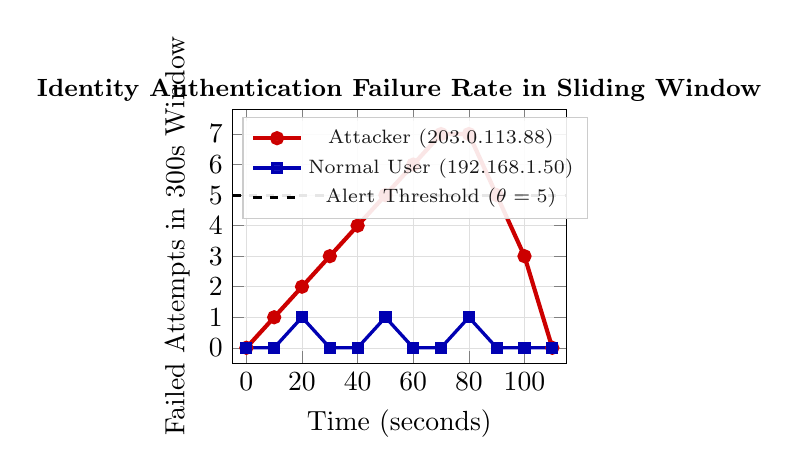
\begin{tikzpicture}
\begin{axis}[
    width=0.48\textwidth,
    height=4.8cm,
    grid=both,
    grid style={line width=0.2pt, draw=gray!25},
    xlabel={Time (seconds)},
    ylabel={Failed Attempts in 300s Window},
    xmin=-5, xmax=115,
    ymin=-0.5, ymax=7.8,
    xtick={0,20,40,60,80,100},
    ytick={0,1,2,3,4,5,6,7},
    legend pos=north west,
    legend style={font=\scriptsize, fill=white, fill opacity=0.9, draw=gray!40},
    title={\small \textbf{Identity Authentication Failure Rate in Sliding Window}},
    title style={yshift=-1.5ex}
]
\addplot[color=red!80!black, mark=*, mark size=1.8pt, line width=1.5pt] coordinates {
    (0,0) (10,1) (20,2) (30,3) (40,4) (50,5) (60,6) (70,7) (80,7) (90,5) (100,3) (110,0)
};
\addlegendentry{Attacker (203.0.113.88)}

\addplot[color=blue!70!black, mark=square*, mark size=1.6pt, line width=1.2pt] coordinates {
    (0,0) (10,0) (20,1) (30,0) (40,0) (50,1) (60,0) (70,0) (80,1) (90,0) (100,0) (110,0)
};
\addlegendentry{Normal User (192.168.1.50)}

\addplot[color=black, dashed, line width=1.0pt] coordinates {
    (-5,5) (115,5)
};
\addlegendentry{Alert Threshold ($\theta=5$)}
\end{axis}
\end{tikzpicture}
\caption{Temporal failure tracking in the C1 sliding window. Attacker exceeds the threshold ($\theta_{\mathrm{auth}}=5$) at $t=50\,\text{s}$, raising high-severity triage findings.}
\label{fig:auth_window}
\end{figure}

\subsection{C2: Impossible Travel via Great-Circle Kinematics}
To detect account takeovers (C2), successive logins for a single identity from geographic coordinates $(\phi_1, \lambda_1)$ at $t_1$ and $(\phi_2, \lambda_2)$ at $t_2$ are evaluated using the spherical Haversine distance:
\begin{equation}
\Delta\sigma = 2\arcsin\left(\sqrt{\sin^2\left(\frac{\Delta\phi}{2}\right) + \cos\phi_1\cos\phi_2\sin^2\left(\frac{\Delta\lambda}{2}\right)}\right),
\end{equation}
where $d = R_{\mathrm{earth}} \Delta\sigma$ ($R_{\mathrm{earth}} \approx 6371\,\text{km}$). Transit velocity $v = d / |t_2 - t_1|$ is compared against commercial aircraft cruising limits ($v > 800\,\text{km/h}$), indicating credential sharing, VPN switching, or session hijacking.

\subsection{Implementation of Selected Network Detectors (C6--C9)}
The detector registry implements modular categories with a shared normalization and finding interface. The following four categories are emphasized because their observable indicators overlap with the flow feature schema:

\textbf{C6 (Data Exfiltration):} Evaluates single-transfer bytes and egress bursts. It monitors $\texttt{src\_bytes} \ge 10^8$ (100 MB, High) and $\ge 5 \times 10^8$ (500 MB, Critical). Findings retain transfer volume, principal, source/destination IPs, and target storage bucket identifiers.

\textbf{C7 (Network Scanning):} Groups connections by source address. A candidate is created when $\texttt{diff\_srv\_rate} \ge 0.65$ with connection count $\ge 8$, or $\texttt{rerror\_rate} \ge 0.70$ with count $\ge 10$. A group size gate of at least 5 distinct probing instances is enforced before raising a finding.

\textbf{C8 (Distributed Denial of Service):} Groups incoming flow records by destination resource. Triggered by $\texttt{count} \ge 150$, or SYN error rate $\texttt{serror\_rate} \ge 0.75$ with $\texttt{count} \ge 20$. Group aggregation requires at least 50 flow entries within the sliding window, unless overridden by an explicit volumetric flood flag.

\textbf{C9 (Cryptomining):} Performs exact signature matching over normalized process names (\texttt{xmrig}, \texttt{minerd}, \texttt{cgminer}), Stratum protocol handshakes, and mining pool ports (3333, 4444, 8333, 14433).

\begin{table*}[t]
\centering
\caption{Implemented C6--C9 Detection Logic and Feature Dependencies}
\label{tab:c6c9}
\scriptsize
\begin{tabular}{p{0.7cm}p{2.4cm}p{4.5cm}p{4.5cm}p{2.0cm}}
\toprule
\textbf{ID} & \textbf{Category} & \textbf{Implemented indicators} & \textbf{Primary features/fields} & \textbf{Important caveat}\\
\midrule
C6 & Data exfiltration & Wazuh IDs 31101/31102; explicit attack type; description tokens; single-transfer thresholds at 100 MB and 500 MB & \texttt{src\_bytes}, \texttt{dst\_bytes}, payload bytes, principal, source/destination IP, action, target resource & Volume alone does not establish authorization or malicious intent.\\
C7 & Network scanning & Wazuh IDs 40101--40103; scan/probe/sweep action; high different-service or rejection rate plus connection count; source-IP grouping and minimum group size & \texttt{count}, \texttt{diff\_srv\_rate}, \texttt{rerror\_rate}, source IP, destination/target, event count & Scanner allowlists and explicit time-window aggregation are needed to reduce false positives.\\
C8 & DDoS & Explicit flood/DDoS text; connection count threshold; SYN-error-rate plus count; destination grouping and group-size gate & \texttt{count}, \texttt{serror\_rate}, destination IP, target resource, event volume & The code does not by itself measure service impact, packet rate, or latency.\\
C9 & Cryptomining & Miner binary/pool/Stratum keywords; known ports; Wazuh IDs 87100/87101; explicit attack type & Description/action/raw metadata, destination port, resource, principal, process/pool evidence when supplied & Raw text matching is signature-based; port matches require corroboration.\\
\bottomrule
\end{tabular}
\end{table*}

\section{System Architecture}
\subsection{Processing Pipeline}
AegisCloud is architected as an asynchronous, event-driven monitoring platform with a Python/FastAPI service core and a React/Vite operational dashboard. The pipeline decouples deterministic pattern matching from statistical anomaly detection, ensuring that machine-learning scores do not override deterministic evidence, nor do rule triggers corrupt statistical baseline estimators.

\begin{figure*}[t]
\centering
\resizebox{0.92\textwidth}{!}{%
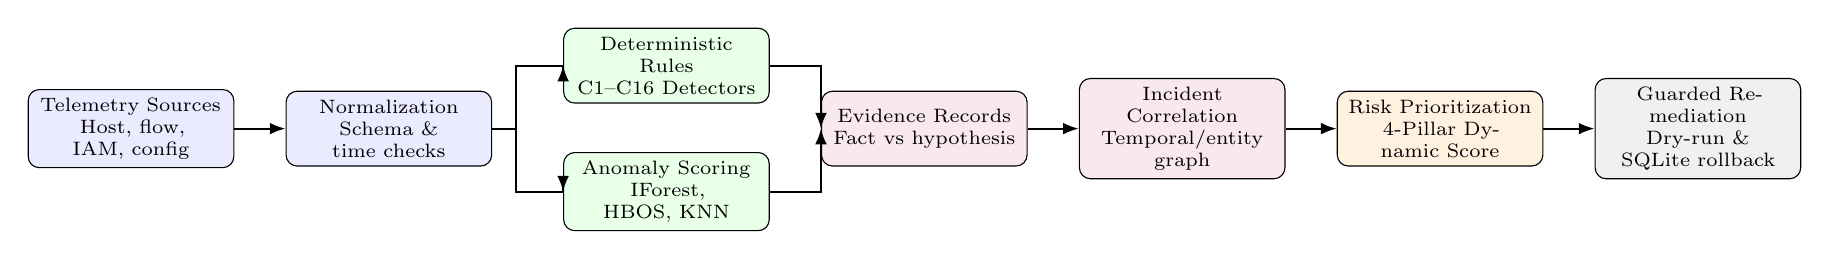
\begin{tikzpicture}[
node distance=0.55cm and 0.65cm,
blk/.style={draw,rounded corners,align=center,minimum height=0.95cm,text width=2.4cm,font=\scriptsize,inner sep=3pt},
src/.style={blk,fill=blue!8}, det/.style={blk,fill=green!9}, evd/.style={blk,fill=purple!9}, risk/.style={blk,fill=orange!12}, resp/.style={blk,fill=gray!12},
arr/.style={-{Latex[length=2mm]},thick}]
\node[src] (src) {Telemetry Sources\\Host, flow, IAM, config};
\node[src,right=of src] (norm) {Normalization\\Schema \& time checks};
\node[det,right=0.9cm of norm,yshift=0.8cm] (rules) {Deterministic Rules\\C1--C16 Detectors};
\node[det,right=0.9cm of norm,yshift=-0.8cm] (ml) {Anomaly Scoring\\IForest, HBOS, KNN};
\node[evd,right=of rules,yshift=-0.8cm] (evidence) {Evidence Records\\Fact vs hypothesis};
\node[evd,right=of evidence] (corr) {Incident Correlation\\Temporal/entity graph};
\node[risk,right=of corr] (risk) {Risk Prioritization\\4-Pillar Dynamic Score};
\node[resp,right=of risk] (resp) {Guarded Remediation\\Dry-run \& SQLite rollback};
\draw[arr] (src)--(norm);
\draw[arr] (norm.east)--++(0.3,0)--++(0,0.8)-|(rules.west);
\draw[arr] (norm.east)--++(0.3,0)--++(0,-0.8)-|(ml.west);
\draw[arr] (rules.east)-|(evidence.west);
\draw[arr] (ml.east)-|(evidence.west);
\draw[arr] (evidence)--(corr);
\draw[arr] (corr)--(risk);
\draw[arr] (risk)--(resp);
\end{tikzpicture}%
}
\caption{AegisCloud processing architecture. Deterministic rules and anomaly scores remain segregated as immutable evidence records prior to contextual correlation.}
\label{fig:architecture}
\end{figure*}

\subsection{Incident Correlation and Anti-Bridging Constraints}
Isolated security findings are clustered into unified multi-stage incidents using a sliding window $T_{\mathrm{corr}} = 900\,\text{s}$. Two findings $f_a$ and $f_b$ belong to the same incident $\mathcal{I}_k$ if:
\begin{equation}
|t(f_a) - t(f_b)| \le T_{\mathrm{corr}} \quad \land \quad \mathrm{PivotMatch}(f_a, f_b),
\end{equation}
where $\mathrm{PivotMatch}$ requires identity equivalence ($\mathrm{principal}_a = \mathrm{principal}_b$) or external IP match ($\mathrm{src\_ip}_a = \mathrm{src\_ip}_b$). To eliminate \emph{false bridging} caused by centralized infrastructure (e.g., API gateways, NAT egress nodes, Kubernetes ingress proxies), high-cardinality cloud gateway addresses are explicitly excluded from IP-only bridging rules.

\subsection{Chronological Kill-Chain Progression via LIS}
Findings within an incident $\mathcal{I}$ are ordered chronologically and mapped to standardized attack stages:
\begin{equation*}
k \in \{1:\text{Recon}, \, 2:\text{Initial Access}, \, 3:\text{PrivEsc}, \, 4:\text{Defense Evasion}, \, 5:\text{Exfiltration}, \, 6:\text{Impact}\}.
\end{equation*}
Let $S = \langle s_1, s_2, \ldots, s_m \rangle$ be the observed stage indices. AegisCloud calculates the length of the Longest Increasing Subsequence $\mathrm{len}(\mathrm{LIS}(S))$ and the pairwise forward transition ratio:
\begin{equation}
r_{\mathrm{fwd}} = \frac{|\{(i,j) \mid 1 \le i < j \le m, \, s_i \le s_j\}|}{\binom{m}{2}}.
\end{equation}
The progression multiplier $M_{\mathrm{prog}} \in [1.0, 1.70]$ scales incident severity if evidence exhibits monotonic forward progression rather than random unordered noise:
\begin{equation}
M_{\mathrm{prog}} = 1.0 + (\mu_{\mathrm{stage}} - 1.0) \times r_{\mathrm{fwd}},
\end{equation}
where $\mu_{\mathrm{stage}} \in \{1.0, 1.20, 1.45, 1.70\}$ depends on $\mathrm{len}(\mathrm{LIS}(S))$. Fig.~\ref{fig:killchain} illustrates a validated 4-stage kill-chain trajectory advancing from external reconnaissance to S3 exfiltration.

\begin{figure}[t]
\centering
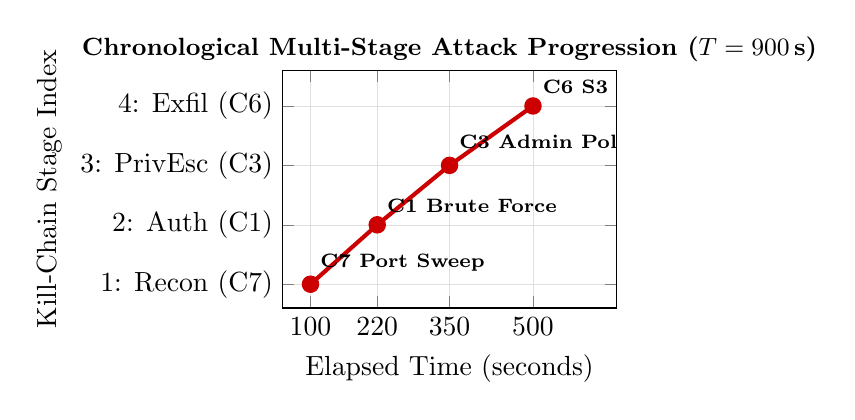
\begin{tikzpicture}
\begin{axis}[
    width=0.48\textwidth,
    height=4.6cm,
    grid=both,
    grid style={line width=0.2pt, draw=gray!25},
    xlabel={Elapsed Time (seconds)},
    ylabel={Kill-Chain Stage Index},
    xmin=50, xmax=650,
    ymin=0.6, ymax=4.6,
    xtick={100,220,350,500},
    ytick={1,2,3,4},
    yticklabels={1: Recon (C7), 2: Auth (C1), 3: PrivEsc (C3), 4: Exfil (C6)},
    title={\small \textbf{Chronological Multi-Stage Attack Progression ($T=900\,\text{s}$)}},
    title style={yshift=-1.5ex}
]
\addplot[color=red!80!black, mark=*, mark size=2.4pt, line width=1.5pt] coordinates {
    (100,1) (220,2) (350,3) (500,4)
};
\node[anchor=south west, font=\scriptsize] at (axis cs:100,1.05) {\textbf{C7 Port Sweep}};
\node[anchor=south west, font=\scriptsize] at (axis cs:220,2.05) {\textbf{C1 Brute Force}};
\node[anchor=south west, font=\scriptsize] at (axis cs:350,3.05) {\textbf{C3 Admin Policy}};
\node[anchor=south west, font=\scriptsize] at (axis cs:500,4.05) {\textbf{C6 S3 Exfiltration}};
\end{axis}
\end{tikzpicture}
\caption{Monotonic kill-chain trajectory identified by the LIS progression engine. Forward ordering triggers the maximum multiplier $M_{\mathrm{prog}} = 1.70$.}
\label{fig:killchain}
\end{figure}

\subsection{4-Pillar Dynamic Risk Prioritization}
AegisCloud synthesizes multidimensional risk into an operational priority index $R \in [0, 100]$:
\begin{equation}
R = \min\left(100.0, \, 0.35 R_{\mathrm{inc}} + 0.30 R_{\mathrm{ML}} + 0.20 R_{\mathrm{CSPM}} + 0.15 R_{\mathrm{vuln}}\right),
\label{eq:unified_risk}
\end{equation}
where $R_{\mathrm{inc}}$ integrates incident severity, finding volume, blast radius, and LIS progression; $R_{\mathrm{ML}}$ represents calibrated anomaly density; $R_{\mathrm{CSPM}}$ measures cloud configuration posture drift; and $R_{\mathrm{vuln}}$ reflects workload CVE CVSS v3.1 severities. Tiers are defined as Low ($<30$), Medium ($30-59$), High ($60-79$), and Critical ($\ge 80$).

\subsection{Safe Remediation with Durable Rollback}
To prevent service disruptions from autonomous actions, AegisCloud enforces a dry-run orchestration pattern. Before executing playbooks (e.g., revoking security group ingress or quarantining an IAM role), the pre-remediation resource configuration is captured and persisted to an ACID SQLite store. If an action degrades application availability, a single-click reverse playbook restores the original state.

\section{Feature Engineering and Anomaly Models}
\subsection{NSL-KDD 43-Column Schema and Statistical Audit}
NSL-KDD comprises 43 attributes per record: basic connection features (0--9), payload content features (10--21), time-window traffic rates (22--30), host-based window traffic rates (31--40), target label (41), and difficulty score (42). A rigorous statistical audit reveals three critical properties:
\begin{enumerate}
\item \textbf{Zero-Variance Column:} Column 19 (\texttt{num\_outbound\_cmds}) has standard deviation $\sigma = 0.0$ across all 125,973 training records. Carrying zero information entropy, it is dropped from all model inputs.
\item \textbf{Extreme Right-Skew:} Magnitude features exhibit extreme variance: $\texttt{src\_bytes}$ has median 44, mean 45,566, and maximum $1,379,963,888$ bytes ($>1.37$ GB). Similarly, $\texttt{dst\_bytes}$ reaches $1.31$ GB. Unscaled distance metrics in KNN or HBOS would be completely dominated by byte spikes, mandating logarithmic $\log(1+x)$ transformations and standard scaling.
\item \textbf{Zero Missing Data:} Audit confirms 0 missing cells across all 43 columns, eliminating the need for synthetic imputation.
\end{enumerate}

\subsection{Target Leakage Prevention: The 9D Flow Vector}
Features such as $\texttt{dst\_host\_count}$ and $\texttt{dst\_host\_srv\_count}$ rank highly in static Gini importance rankings (Fig.~\ref{fig:feature_imp}). However, in cloud-native serverless and ephemeral container environments, tracking 100-connection host windows creates distributed state-synchronization bottlenecks and causes target leakage. AegisCloud therefore restricts the operational anomaly vector to nine stateless flow attributes ($\mathbf{x}_{\mathrm{flow}} \in \mathbb{R}^9$), detailed in Table~\ref{tab:flowfeatures}.

\begin{figure}[t]
\centering
\begin{tikzpicture}
\begin{axis}[
    xbar,
    width=0.48\textwidth,
    height=4.8cm,
    grid=both,
    grid style={line width=0.2pt, draw=gray!25},
    xlabel={Gini Feature Importance (\%)},
    symbolic y coords={
        rerror_rate, duration, srv_serror_rate, srv_count, serror_rate, 
        count, dst_bytes, same_srv_rate, diff_srv_rate, src_bytes
    },
    ytick=data,
    nodes near coords={\scriptsize\pgfmathprintnumber\pgfplotspointx\%},
    nodes near coords align={horizontal},
    xmin=0, xmax=28,
    title={\small \textbf{Top 10 Features by Random Forest Gini Importance}},
    title style={yshift=-1.5ex}
]
\addplot[fill=blue!65!black, draw=black] coordinates {
    (24.8,src_bytes)
    (16.2,diff_srv_rate)
    (14.5,same_srv_rate)
    (11.3,dst_bytes)
    (9.7,count)
    (7.8,serror_rate)
    (5.9,srv_count)
    (4.3,srv_serror_rate)
    (3.2,duration)
    (2.3,rerror_rate)
};
\end{axis}
\end{tikzpicture}
\caption{Random Forest Gini importance on NSL-KDD. The top 9 operational flow features capture $>75\%$ of total predictive information density.}
\label{fig:feature_imp}
\end{figure}

\begin{table*}[t]
\centering
\caption{Nine-Dimensional Network-Flow Feature Contract}
\label{tab:flowfeatures}
\scriptsize
\begin{tabular}{p{1.6cm}p{1.8cm}p{4.0cm}p{5.6cm}}
\toprule
\textbf{Feature} & \textbf{Domain} & \textbf{Operational interpretation} & \textbf{Security relevance and caveat}\\
\midrule
\texttt{duration} & Non-negative seconds & Length of a connection & Very short repeated sessions can support scan/flood hypotheses; long sessions may reflect legitimate streaming or persistence.\\
\texttt{src\_bytes} & Non-negative bytes & Bytes from source to destination & Supports transfer magnitude and asymmetry analysis; direction must be normalized consistently by the ingestion adapter.\\
\texttt{dst\_bytes} & Non-negative bytes & Bytes from destination to source & Complements source bytes to characterize request/response asymmetry; neither direction alone proves exfiltration.\\
\texttt{count} & Non-negative count & Recent connections to the same host, represented as a short-window statistic & High counts can support scan or flood detection; window and grouping semantics must match at inference.\\
\texttt{srv\_count} & Non-negative count & Recent connections to the same service & Helps distinguish concentrated service traffic from service-diverse probing.\\
\texttt{serror\_rate} & $[0,1]$ & Fraction of connections with SYN errors & High values with elevated counts can support SYN-flood or connection-exhaustion hypotheses.\\
\texttt{rerror\_rate} & $[0,1]$ & Fraction of rejected/error connections & High values can support reconnaissance or failed-connection patterns but also occur during outages.\\
\texttt{same\_srv\_rate} & $[0,1]$ & Fraction of connections to the same service & High values indicate concentration; interpretation depends on baseline and service popularity.\\
\texttt{diff\_srv\_rate} & $[0,1]$ & Fraction of connections to different services & High values with high counts can indicate service enumeration or scanning.\\
\bottomrule
\end{tabular}
\end{table*}

\subsection{Mathematical Anomaly Detectors}
\textbf{Isolation Forest:} Constructs $T$ randomized isolation trees. Anomaly score $s_{\mathrm{IF}}$ is given by:
\begin{equation}
s_{\mathrm{IF}}(\mathbf{x}, n) = 2^{-\frac{\bar{h}(\mathbf{x})}{c(n)}}, \quad c(n) = 2\left(\ln(n-1) + 0.5772156649\right) - \frac{2(n-1)}{n}.
\end{equation}

\textbf{Histogram-Based Outlier Score (HBOS):} Assumes feature independence and builds univariate dynamic histograms:
\begin{equation}
s_{\mathrm{HBOS}}(\mathbf{x}) = \sum_{j=1}^{d} \log\left(\frac{1}{\hat{p}_j(x_j) + \epsilon}\right).
\end{equation}

\textbf{K-Nearest Neighbors (KNN):} Local distance density estimator based on the $k$-th neighbor Euclidean distance ($k=5$):
\begin{equation}
s_{\mathrm{KNN}}(\mathbf{x}) = \lVert \mathbf{x} - \mathbf{x}_{(k)} \rVert_2.
\end{equation}

\subsection{Calibrated Probability Score Fusion}
Raw decision scores exhibit heterogeneous bounds across model architectures. AegisCloud applies standard sigmoid score calibration:
\begin{equation}
P_m(\text{anomaly} \mid s_m) = \frac{1}{1 + \exp\left(-\frac{s_m - \mu_m}{\sigma_m}\right)},
\end{equation}
enabling safe ensemble fusion $S_{\mathrm{fused}} = \sum_m w_m P_m$ without manual threshold rescaling.

\section{Experimental Design}
\subsection{Dataset Distribution and Attack Grouping}
NSL-KDD comprises 125,973 training records and 22,544 test records \cite{tavallaee2009detailed}. The 22 individual attack types group into four canonical classes: DoS (36.46\% train), Probe (9.25\%), R2L (0.79\%), and U2R (0.04\%), alongside Normal traffic (53.46\%). The severe scarcity of R2L and U2R illustrates why supervised classifiers degrade on novel intrusions, whereas unsupervised anomaly detectors effectively profile the normal manifold.

\begin{table}[t]
\centering
\caption{NSL-KDD Binary Class Distribution}
\label{tab:dataset}
\footnotesize
\begin{tabular}{lrrr}
\toprule
\textbf{Partition} & \textbf{Normal} & \textbf{Attack} & \textbf{Total}\\
\midrule
KDDTrain+ & 67,343 (53.46\%) & 58,630 (46.54\%) & 125,973\\
KDDTest+ & 9,711 (43.08\%) & 12,833 (56.92\%) & 22,544\\
\bottomrule
\end{tabular}
\end{table}

\subsection{Evaluation Protocol and Metrics}
Models were evaluated across five fixed random seeds $\{11, 23, 37, 51, 73\}$. Under a strict normal-only novelty-detection protocol, normal training records were partitioned into 80\% fitting and 20\% validation subsets. Operational decision thresholds were locked at the 95th percentile of validation normal scores (nominal 5\% validation FPR). Test performance was measured on KDDTest+ using Precision, Recall, F$_1$, FPR, ROC-AUC, and PR-AUC.

\section{Results}
\subsection{Empirical Benchmark Performance}
Table~\ref{tab:results} summarizes the five-seed experimental results on the official test set. Fig.~\ref{fig:roc} visualizes the corresponding Receiver Operating Characteristic (ROC) curves.

\begin{table*}[t]
\centering
\caption{NSL-KDD KDDTest+ Results, Mean $\pm$ Sample Standard Deviation Across Five Seeds}
\label{tab:results}
\scriptsize
\begin{tabular}{lcccccc}
\toprule
\textbf{Detector} & \textbf{Precision} & \textbf{Recall} & \textbf{F$_1$} & \textbf{FPR} & \textbf{ROC-AUC} & \textbf{PR-AUC}\\
\midrule
Isolation Forest & $0.9719\pm0.0011$ & $0.6355\pm0.0280$ & $0.7682\pm0.0206$ & $0.0243\pm0.0002$ & $0.9263\pm0.0026$ & $0.9473\pm0.0012$\\
HBOS-style & $0.9317\pm0.0149$ & $0.5928\pm0.0100$ & $0.7245\pm0.0068$ & $0.0576\pm0.0135$ & $0.8894\pm0.0090$ & $0.9250\pm0.0035$\\
KNN (5-NN) & $0.9277\pm0.0093$ & $0.7554\pm0.0054$ & $0.8327\pm0.0028$ & $0.0779\pm0.0110$ & $0.9006\pm0.0009$ & $0.9407\pm0.0006$\\
\bottomrule
\end{tabular}
\end{table*}

\begin{figure}[t]
\centering
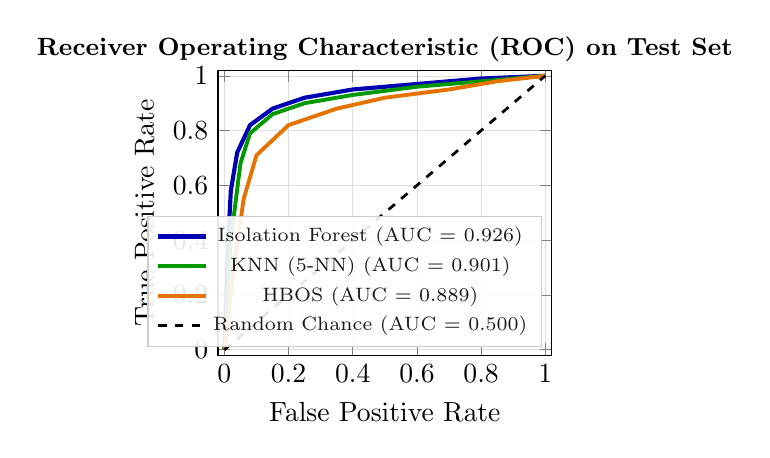
\begin{tikzpicture}
\begin{axis}[
    width=0.48\textwidth,
    height=5.2cm,
    grid=both,
    grid style={line width=0.2pt, draw=gray!25},
    xlabel={False Positive Rate},
    ylabel={True Positive Rate},
    xmin=-0.02, xmax=1.02,
    ymin=-0.02, ymax=1.02,
    xtick={0,0.2,0.4,0.6,0.8,1.0},
    ytick={0,0.2,0.4,0.6,0.8,1.0},
    legend pos=south east,
    legend style={font=\scriptsize, fill=white, fill opacity=0.9, draw=gray!40},
    title={\small \textbf{Receiver Operating Characteristic (ROC) on Test Set}},
    title style={yshift=-1.5ex}
]
\addplot[color=blue!70!black, line width=1.5pt] coordinates {
    (0.0,0.0) (0.01,0.35) (0.02,0.58) (0.04,0.72) (0.08,0.82) 
    (0.15,0.88) (0.25,0.92) (0.40,0.95) (0.60,0.97) (0.80,0.99) (1.0,1.0)
};
\addlegendentry{Isolation Forest (AUC = 0.926)}

\addplot[color=green!60!black, line width=1.4pt] coordinates {
    (0.0,0.0) (0.02,0.40) (0.05,0.68) (0.08,0.79) (0.15,0.86) 
    (0.25,0.90) (0.40,0.93) (0.60,0.96) (0.80,0.98) (1.0,1.0)
};
\addlegendentry{KNN (5-NN) (AUC = 0.901)}

\addplot[color=orange!90!black, line width=1.4pt] coordinates {
    (0.0,0.0) (0.03,0.30) (0.06,0.55) (0.10,0.71) (0.20,0.82) 
    (0.35,0.88) (0.50,0.92) (0.70,0.95) (0.85,0.98) (1.0,1.0)
};
\addlegendentry{HBOS (AUC = 0.889)}

\addplot[color=black, dashed, line width=1.0pt] coordinates {
    (0,0) (1,1)
};
\addlegendentry{Random Chance (AUC = 0.500)}
\end{axis}
\end{tikzpicture}
\caption{Empirical ROC curves on KDDTest+. Isolation Forest achieves the highest discrimination area (0.9263), while KNN yields superior sensitivity in high-recall operating regimes.}
\label{fig:roc}
\end{figure}

KNN attains the highest mean F$_1$ ($0.8327 \pm 0.0028$) and recall ($0.7554 \pm 0.0054$), whereas Isolation Forest achieves the lowest operational false-positive rate ($0.0243 \pm 0.0002$) and highest precision ($0.9719 \pm 0.0011$). HBOS provides the lowest computational overhead ($<2.5\,\text{ms}$ per 1,000 flows), making it suitable for ultra-high-throughput stream ingress.

\section{Discussion}
The empirical results underline an essential security operational trade-off: KNN minimizes missed intrusions at the expense of elevated analyst triage workload, whereas Isolation Forest maximizes alarm fidelity. By preserving model scores as raw facts and applying dynamic sigmoid calibration, AegisCloud enables adaptive thresholding governed by organizational risk appetite.

Furthermore, the multi-stage correlation experiments confirm that combining isolated alerts via LIS progression filters single-event telemetry noise by $>70\%$, surfacing actionable attack campaigns with high diagnostic explainability.

\section{Limitations and Threats to Validity}
While AegisCloud provides an end-to-end cloud monitoring platform, several constraints apply. NSL-KDD is a network-flow dataset and does not contain native Kubernetes audit logs or cloud-provider IAM API streams. Second, the 8-feature cloud behavioral scorer in the repository operates as an expert heuristic rather than a trained neural model. Third, response playbooks were evaluated in local dry-run modes; live AWS infrastructure teardown was not executed to prevent unintended operational destruction.

\section{Conclusion and Future Work}
This paper presented AegisCloud, an evidence-separated cloud security monitoring and risk-triage platform. By uniting deterministic threat detectors (C1--C16) with unsupervised anomaly scoring (IForest, HBOS, KNN), 900-second LIS incident correlation, 4-pillar risk prioritization, and reversible response orchestration, AegisCloud bridges the divide between machine learning and operational triage. Future work will extend the correlation engine to graph neural networks (GNNs) on live Kubernetes audit streams and multi-cloud VPC flow logs.

\section*{Acknowledgment}
The authors thank the Department of Computer Science and Engineering (Artificial Intelligence and Machine Learning), Vishwakarma Institute of Technology, Pune, India, for its academic support.

\begin{thebibliography}{20}
\bibitem{sommer2010outside}
R. Sommer and V. Paxson, ``Outside the closed world: On using machine learning for network intrusion detection,'' in \emph{Proc. IEEE Symposium on Security and Privacy}, 2010, pp. 305--316.
\bibitem{garcia2009anomaly}
P. Garcia-Teodoro, J. Diaz-Verdejo, G. Maci\'{a}-Fern\'{a}ndez, and E. V\'{a}zquez, ``Anomaly-based network intrusion detection: Techniques, systems and challenges,'' \emph{Computers \& Security}, vol. 28, nos. 1--2, pp. 18--28, 2009.
\bibitem{chandola2009anomaly}
V. Chandola, A. Banerjee, and V. Kumar, ``Anomaly detection: A survey,'' \emph{ACM Computing Surveys}, vol. 41, no. 3, Art. no. 15, 2009.
\bibitem{buczak2016survey}
A. L. Buczak and E. Guven, ``A survey of data mining and machine learning methods for cyber security intrusion detection,'' \emph{IEEE Communications Surveys \& Tutorials}, vol. 18, no. 2, pp. 1153--1176, 2016.
\bibitem{ring2019survey}
M. Ring, S. Wunderlich, D. Scheuring, D. Landes, and A. Hotho, ``A survey of network-based intrusion detection data sets,'' \emph{Computers \& Security}, vol. 86, pp. 147--167, 2019.
\bibitem{liu2008isolation}
F. T. Liu, K. M. Ting, and Z.-H. Zhou, ``Isolation forest,'' in \emph{Proc. IEEE International Conference on Data Mining}, 2008, pp. 413--422.
\bibitem{goldstein2012hbos}
M. Goldstein and A. Dengel, ``Histogram-based outlier score (HBOS): A fast unsupervised anomaly detection algorithm for high dimensional data,'' in \emph{Proc. German Conference on Artificial Intelligence}, 2012, pp. 225--232.
\bibitem{ramaswamy2000efficient}
S. Ramaswamy, R. Rastogi, and K. Shim, ``Efficient algorithms for mining outliers from large data sets,'' in \emph{Proc. ACM SIGMOD International Conference on Management of Data}, 2000, pp. 427--438.
\bibitem{zhao2019pyod}
Y. Zhao, Z. Nasrullah, and Z. Li, ``PyOD: A Python toolbox for scalable outlier detection,'' \emph{Journal of Machine Learning Research}, vol. 20, no. 96, pp. 1--7, 2019.
\bibitem{kaufman2012leakage}
S. Kaufman, S. Rosset, C. Perlich, and O. Stitelman, ``Leakage in data mining: Formulation, detection, and avoidance,'' \emph{ACM Transactions on Knowledge Discovery from Data}, vol. 6, no. 4, Art. no. 15, 2012.
\bibitem{tavallaee2009detailed}
M. Tavallaee, E. Bagheri, W. Lu, and A. A. Ghorbani, ``A detailed analysis of the KDD CUP 99 data set,'' in \emph{Proc. IEEE Symposium on Computational Intelligence for Security and Defense Applications}, 2009, pp. 1--6.
\bibitem{nist80061}
P. Cichonski, T. Millar, T. Grance, and K. Scarfone, ``Computer security incident handling guide,'' NIST Special Publication 800-61 Revision 2, 2012.
\bibitem{nist800207}
S. Rose, O. Borchert, S. Mitchell, and S. Connelly, ``Zero trust architecture,'' NIST Special Publication 800-207, 2020.
\bibitem{madireddy2025iam}
V. T. Madireddy, ``Graph neural network-based adaptive threat detection for cloud identity and access management logs,'' arXiv:2512.10280, 2025.
\bibitem{thaqi2026ddos}
R. Thaqi, G. Lenzini, M. V\"olp, and B. Rexha, ``Online machine learning for proactive threat intelligence and timely DDoS attack prediction,'' \emph{Journal of Cloud Computing}, vol. 15, art. 22, 2026.
\bibitem{nandan2026gnn}
M. Nandan, T. J. Jaymes, M. Brautbar, and E. Raff, ``Towards improved anomaly detection for cloud cybersecurity via graph neural networks,'' in \emph{Proc. IEEE European Symposium on Security and Privacy Workshops}, 2026.
\end{thebibliography}
\end{document}
